\documentclass[twocolumn,a4paper]{article}
\usepackage{graphicx}
\usepackage{subfigure}
\usepackage{amsfonts}
\usepackage{color}
\usepackage{lineno}
\setlength{\columnsep}{10pt}
\setlength{\oddsidemargin}{0pt}
\setlength{\topmargin}{0pt}
\setlength{\headheight}{0pt}
\setlength{\headsep}{0pt}
\setlength{\marginparsep}{0pt}
\setlength{\marginparwidth}{0pt}
\addtolength{\voffset}{-50pt}
\setlength{\textheight}{26.8cm}
\author{Siwang Li}

\title{Report of Material Optimization} 

%% document begin here
\begin{document}
\maketitle

\section{Definitions}
In the following, we use $u,y,z$ to denote the displacements in full space, the
RS coordinates, and the reduced coordinates, and $r$ is the dimension of the
reduced coordinates. And we define the mapping functions between these
coordinates as $u=T(y)$, $y=T^{-1}(u)$, $y=\hat{W}z$, and $y=\hat{W}^{-p}z$.
\section{Experiments}
In the first experiment, we use a beam with one end is constrained, and compute
$\hat{W}$ with these constraints considered. Given an initial shape $u0$ as
shown in figure \ref{input1}, we set $z0=\hat{W}^{-p}T^{-1}(u0)$, and $v0=0$, and
use an implicit integrator to obtain $z_1,\cdots,z_{100}$. Here, $r=10$. Then we
compute $y_i=\hat{W}z_i$,$u_i=T(y_i)$, $y'_i=T^{-1}(u_i)$,
$z'_i=\hat{W}^{-p}y'_i$ , and obtain the following results
\begin{itemize}
\item $\|\hat{W}^{-p}\hat{W}-I\| < 10^{-14}$, $\|\hat{W}^{-p}y_i-z_i\|/\|z_i\| <
  10^{-14}$.
\item For $i\in[0,8]$, $\|y_i-y_i'\|/\|y_i\|>1.3$, and for $i\in[9,100]$,
  $\|y_i-y_i'\|/\|y_i\|\approx 0.01$.
\item For $i\in[0,8]$, $\|z_i-z_i'\|/\|z_i\|>0.2$, and for $i\in[9,100]$,
  $\|z_i-z_i'\|/\|z_i\|\approx 0.0005$.
\item The pictures of each mode of $z$ and $z'$ are displayed at \ref{zzc}. The
  smooth ones are $z$.
\item We use $z_{20},\cdots,z_{100}$ to approximate $K$, $D$,diagonalize $K$ to
  obtain the eigenvalues are $(-11, -39, -14, 0.049, 0.17, 1.6, 4.3, 5.5, 15,
  1158)$. And the correct eigenvalues should be $(0.049, 0.15, 1.6, 4.2, 5.1,
  8.6, 12, 28,39, 45)$.
\end{itemize}
\begin{figure}
  \centering
  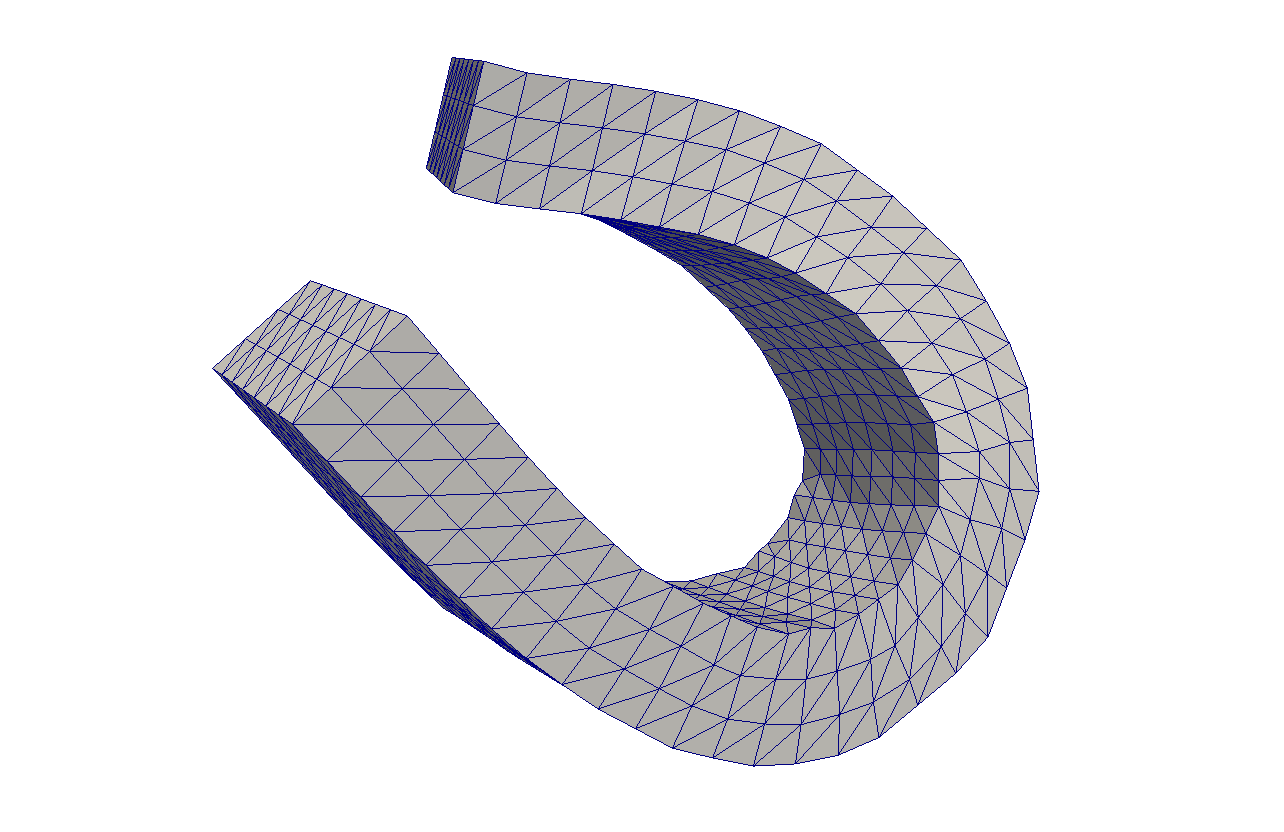
\includegraphics[width=0.4\textwidth]{./figures/rscon_input.png}
  \caption{The initial shape for the first experiment.}
  \label{input1}
\end{figure}
\begin{figure}
  \centering
  \subfigure[mode 1,2,3] { \label{fig:a} 
  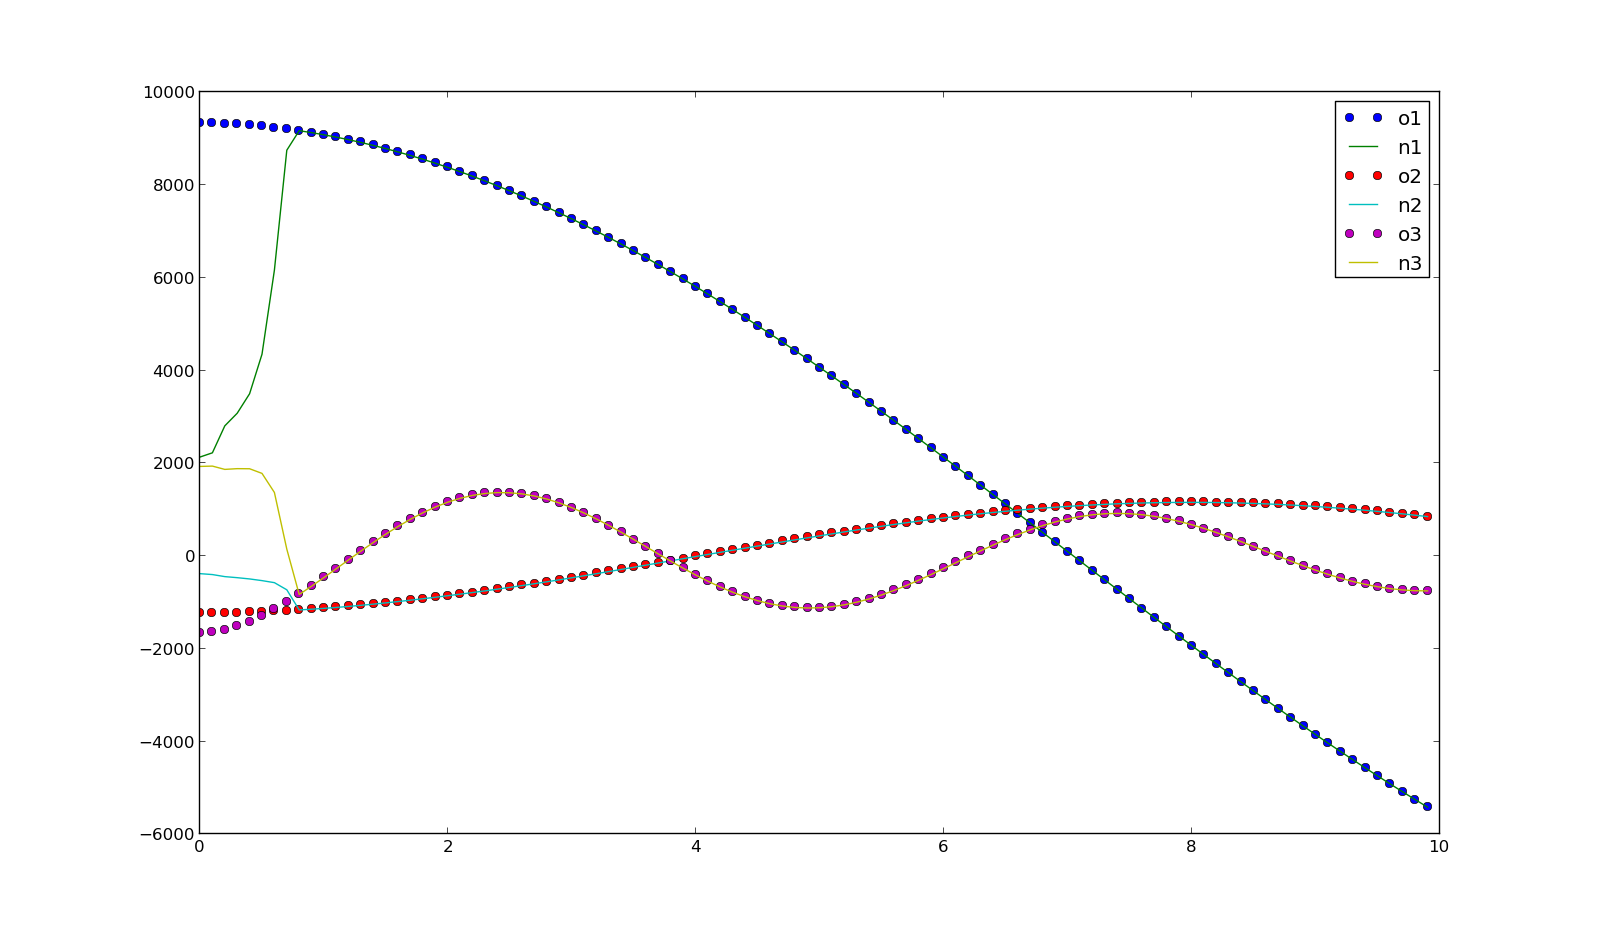
\includegraphics[width=0.48\textwidth]{./figures/rsmode1-3.png}
  }
  \subfigure[mode 4,5,6] { \label{fig:b} 
    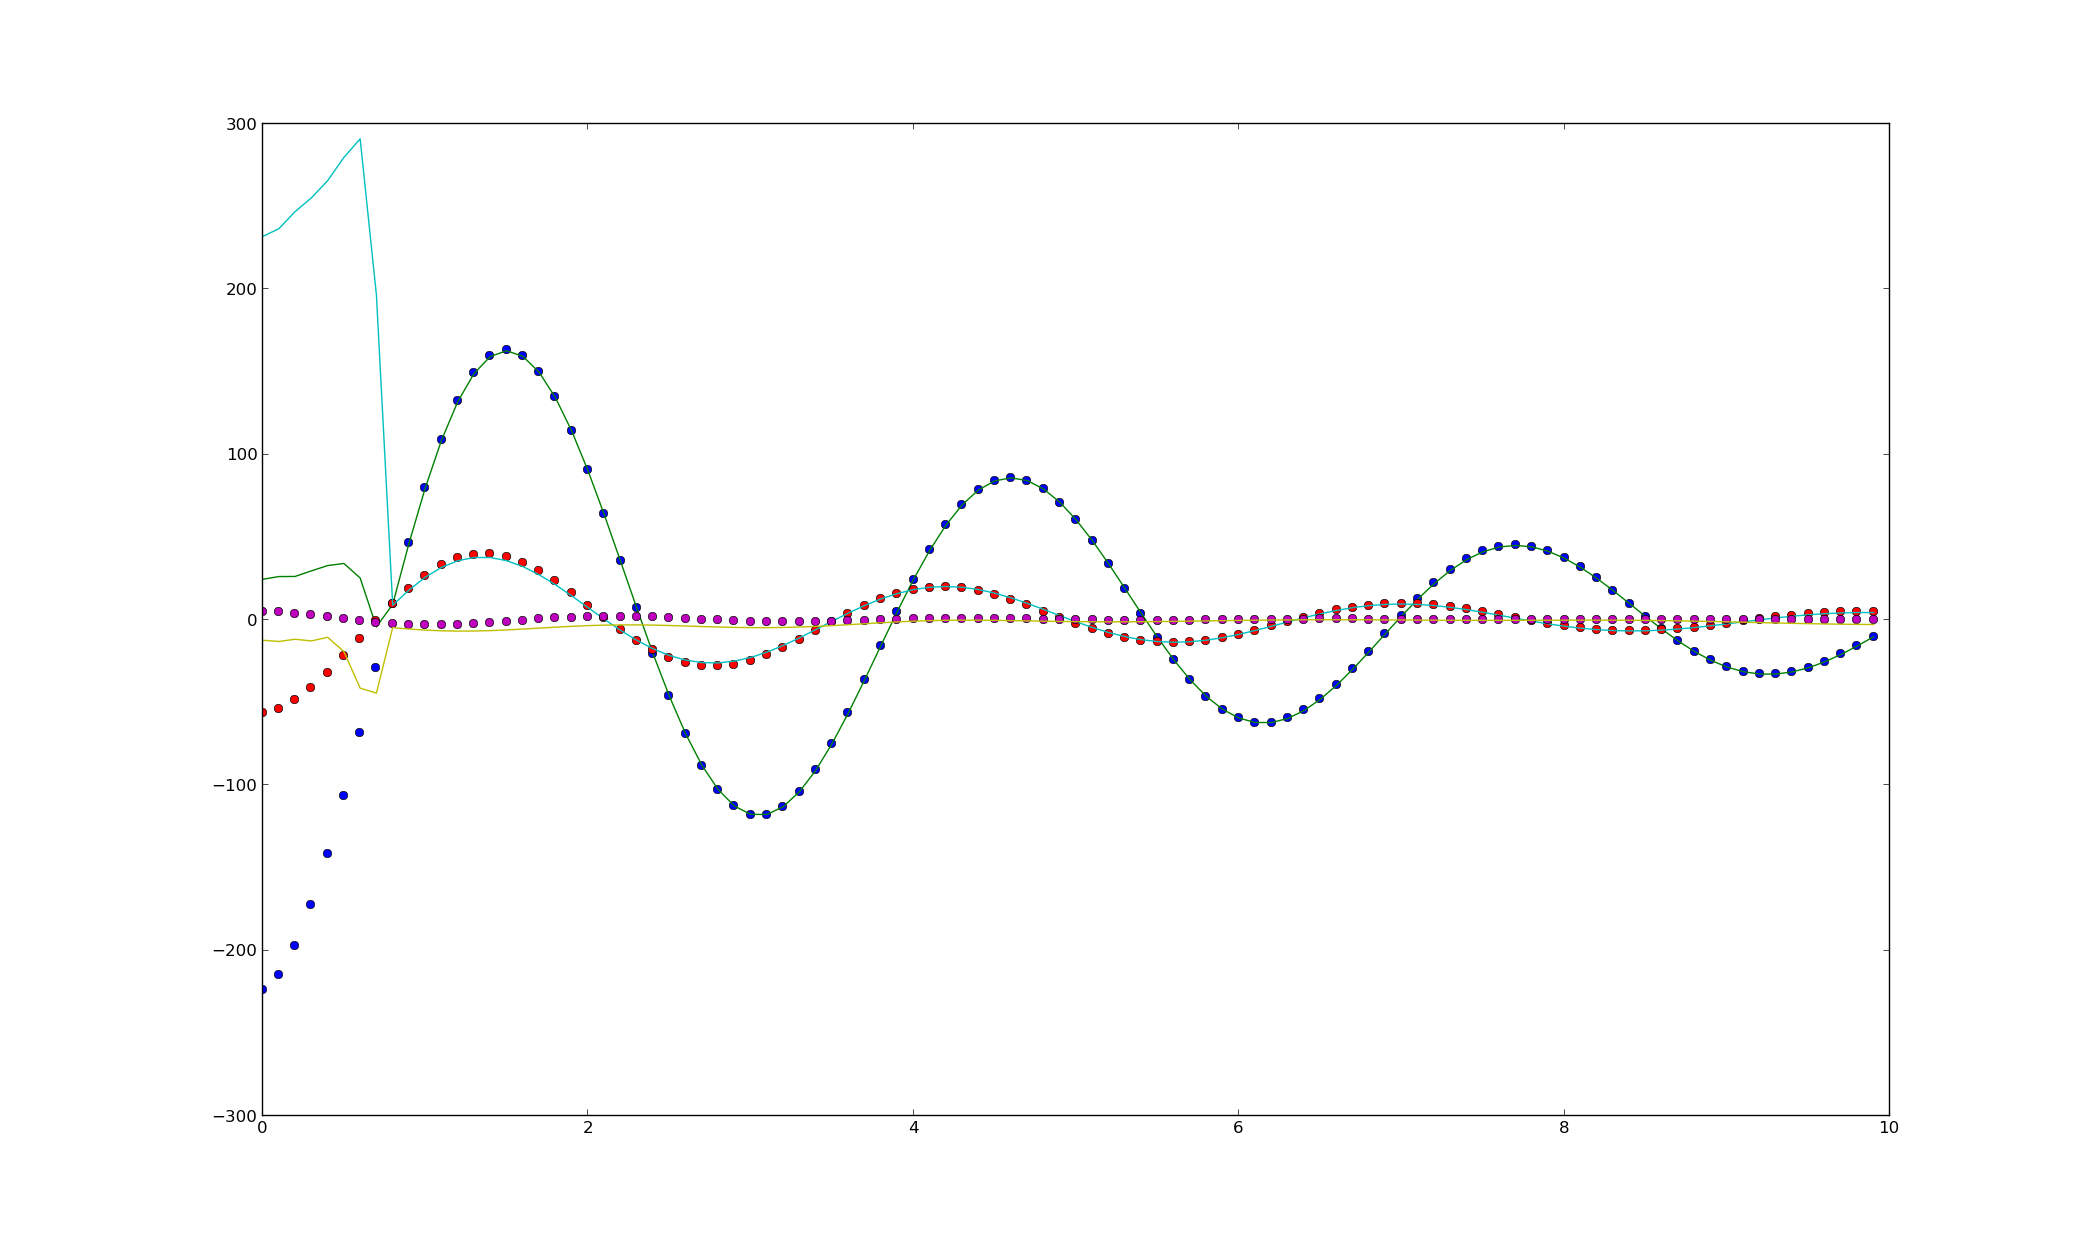
\includegraphics[width=0.48\textwidth]{./figures/rsmode4-6.png}
  }
  \subfigure[mode 7,8,9] { \label{fig:b} 
    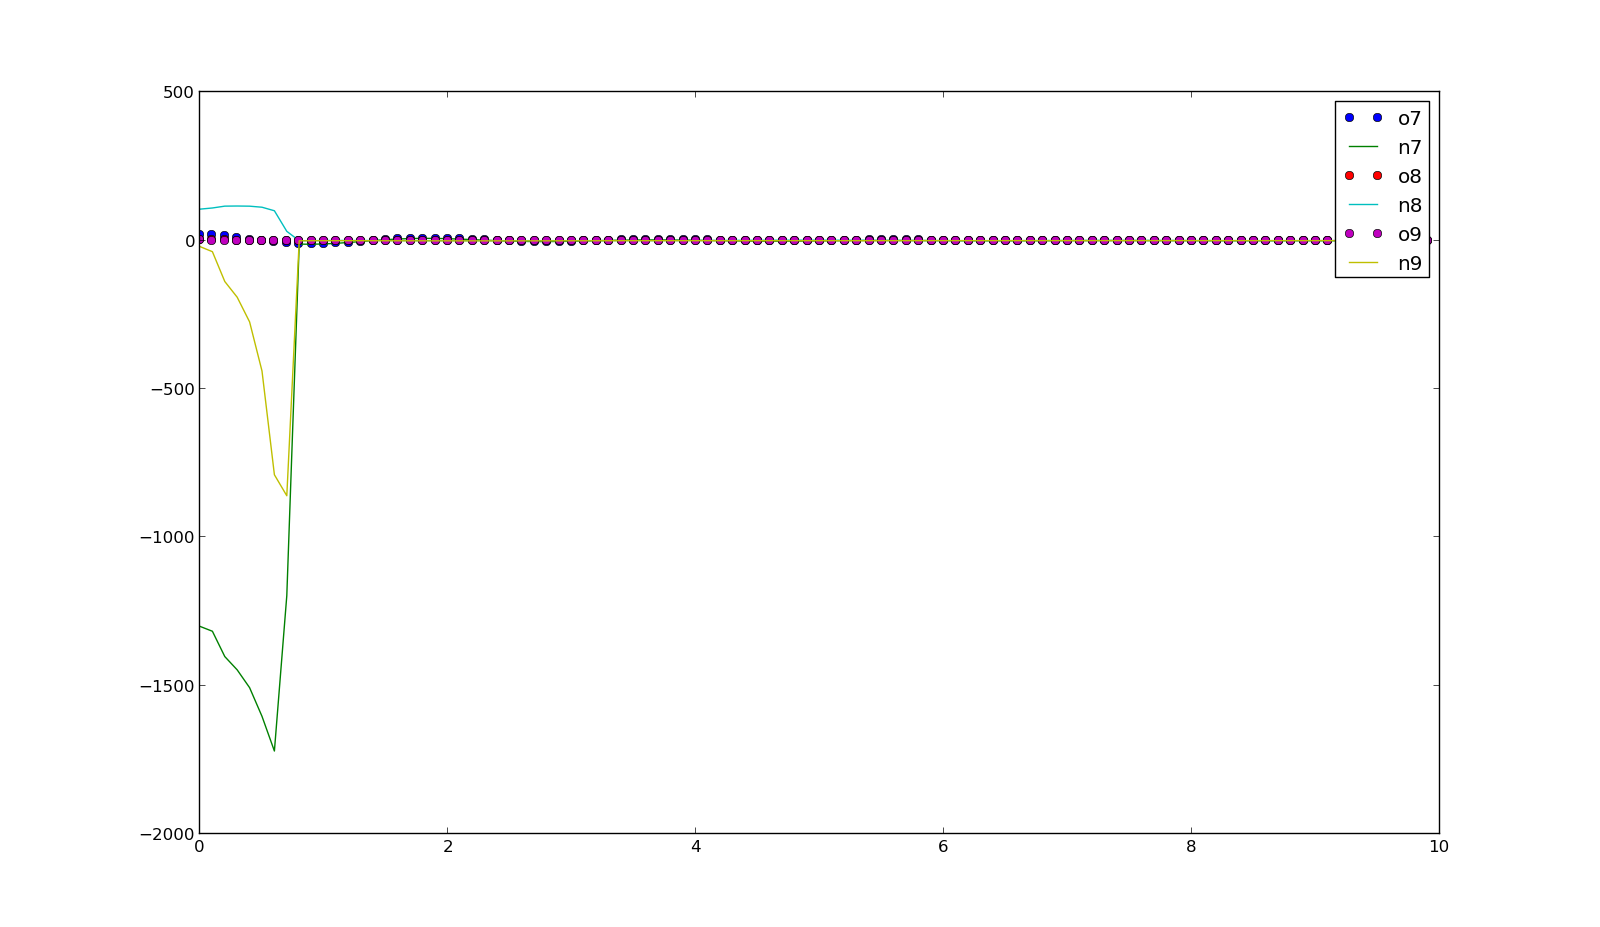
\includegraphics[width=0.48\textwidth]{./figures/rsmode7-9.png}
  }
  \caption{Points are $z$, and others are $z'$. Time step is $0.1$, and there is
  100 frames here. They are almost overlapped for $i>8$.}
  \label{zzc}.
\end{figure}

The second experiment is similar to the above, except that we constrained the
barycenter of the beam only. We found $\|\hat{W}^{-p}\hat{W}-I\|=0.12$,
$\|\hat{W}^{-p}y_i-z_i\|/\|z_i\|\approx 0.002$,
$\|\hat{W}^{-p}\|=5\times10^{15}$, and we failed to solve $K$.

\section{Analysis}
We explained some of the results here. 
\begin{itemize}
\item When frame $i<8$, $\|y_i-y_i'\|/\|y_i\|$ and $\|z_i-z_i'\|/\|z_i\|$ are
  large. This is because when we compute $log(R)$, for the frame $i<8$, the
  angles of some tetrahedrons are near $\pi$, and the rotation vector of $y_i$
  in the near tetrahedron may have opposite sign, and result in incorrect $y_i$
  and $z_i$.
\item Even though we use $z_{20},\cdots,z_{100}$ to approximate $K$, the
  resulting eigenvalues are significantly different from the ground truth. This
  is because, for $z_{20},\cdots,z_{100}$, there are also some modes that are
  greately differs from $z'_{20},\cdots,z'_{100}$, and as $K$ is dense, these
  modes will significantly effect the approximation of other modes. Actually, in
  this experiment, if we use a diagnal $K$ for approximatation, the results will
  be better(the first 5 modes will approximate quite well).
\end{itemize}

\section{DFT}
We apply DFT on each mode of the input $z'$, and the results of mode $1-8$ are
shown in figure 3. However, we found that the frequence with the largest
magnitude is not coincide with the frequence compute from the correct
eigenvalues.

\section{Conclusion}
Even the input animation are generated using RS method, there are several
problems have not been solved yet:
\begin{itemize}
\item To compute the RS coordinates $y$ from $u$ correctly, we need to carefully
  treat the case of rotation angles near $\pi$ of some tetrahedrons.
\item Even the above problem has been solved, the reduced coordinates $z_i$ may
  still differs from the input one $z'_i$, especially for the modes will large
  eigenvalues. And as we use a dense $K$, all modes are coupled, and these
  incorrect $z_i$ will significantly effect the approximation of other
  modes. Then the results will greately differs from the ground truth.
\end{itemize}

Thus, for the general case, where the input animation are not generated by RS
method, the approximation would be much harder.
\begin{figure*}
  \centering
  \subfigure[mode 1] { \label{fig:a} 
    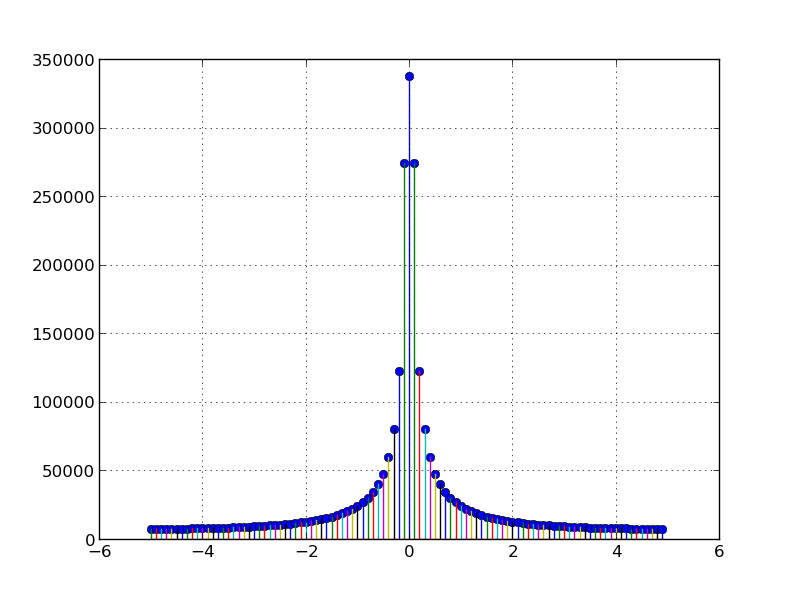
\includegraphics[width=0.48\textwidth]{./figures/DFT_mode_0.png}
  }
  \subfigure[mode 2] { \label{fig:b} 
    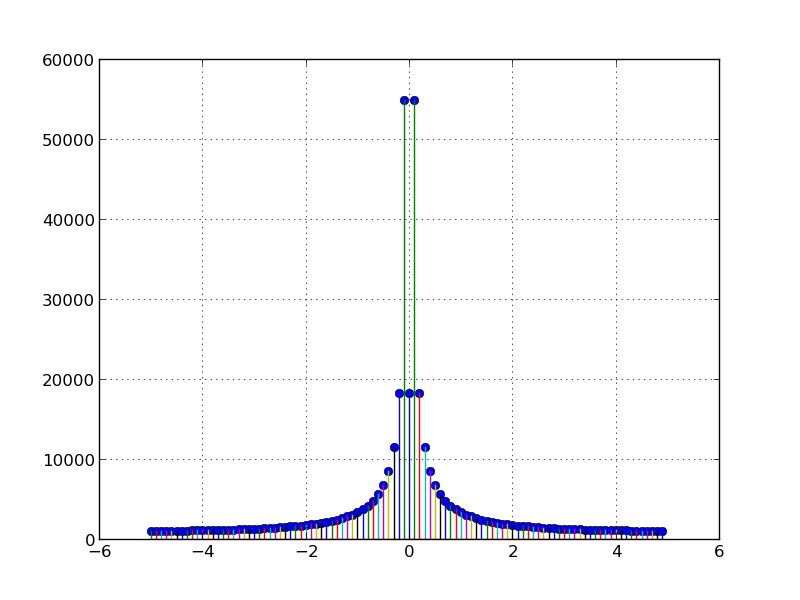
\includegraphics[width=0.48\textwidth]{./figures/DFT_mode_1.png}
  }
  \subfigure[mode 3] { \label{fig:b} 
    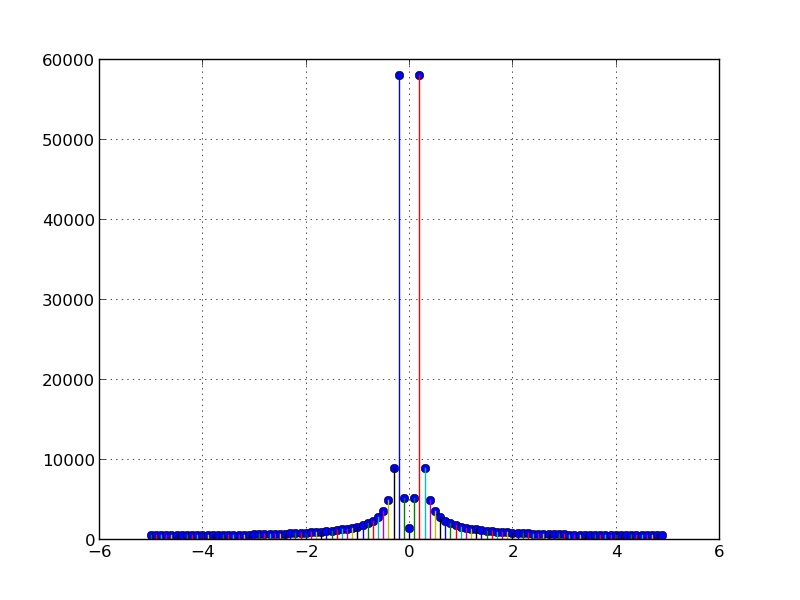
\includegraphics[width=0.48\textwidth]{./figures/DFT_mode_2.png}
  }
  \subfigure[mode 4] { \label{fig:a} 
    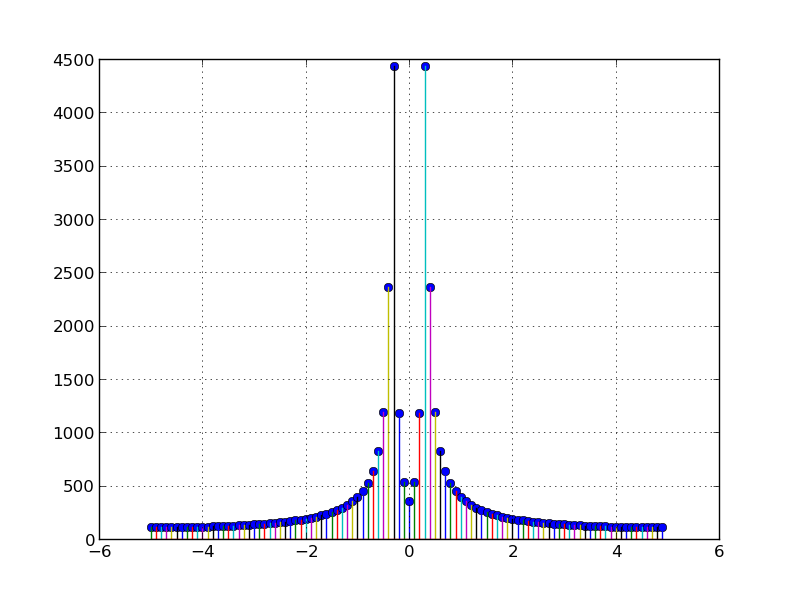
\includegraphics[width=0.48\textwidth]{./figures/DFT_mode_3.png}
  }
  \subfigure[mode 5] { \label{fig:b} 
    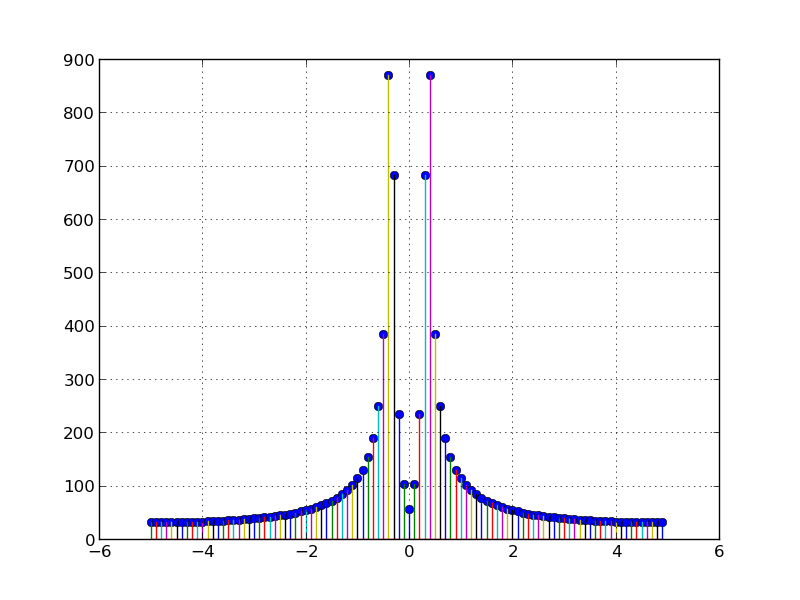
\includegraphics[width=0.48\textwidth]{./figures/DFT_mode_4.png}
  }
  \subfigure[mode 6] { \label{fig:b} 
    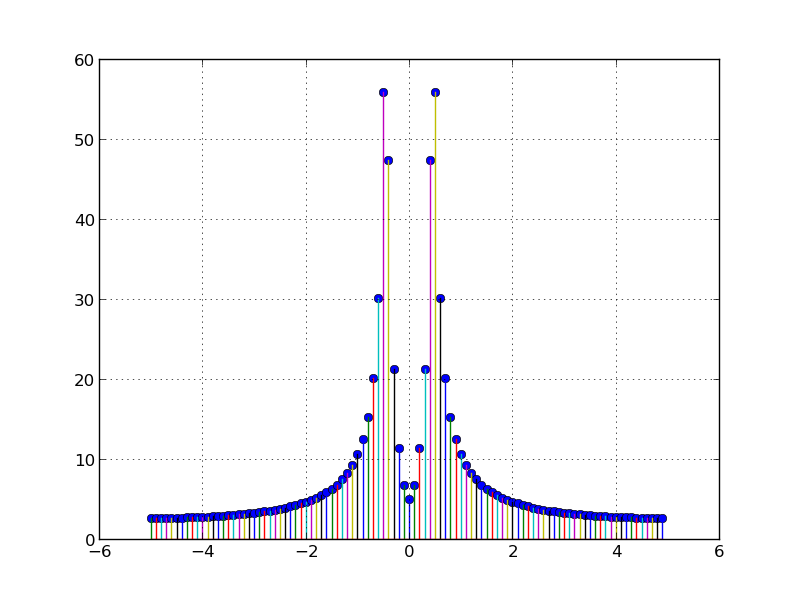
\includegraphics[width=0.48\textwidth]{./figures/DFT_mode_5.png}
  }
  \subfigure[mode 7] { \label{fig:a} 
    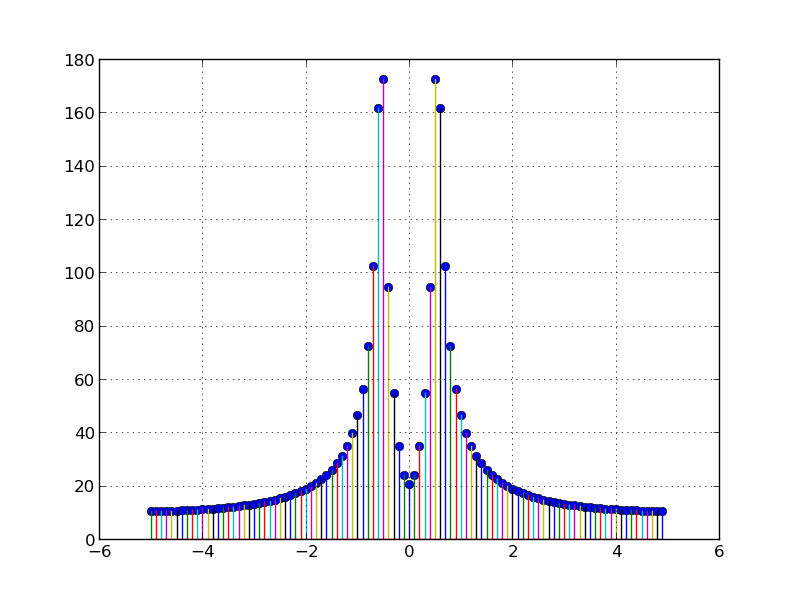
\includegraphics[width=0.48\textwidth]{./figures/DFT_mode_6.png}
  }
  \subfigure[mode 8] { \label{fig:b} 
    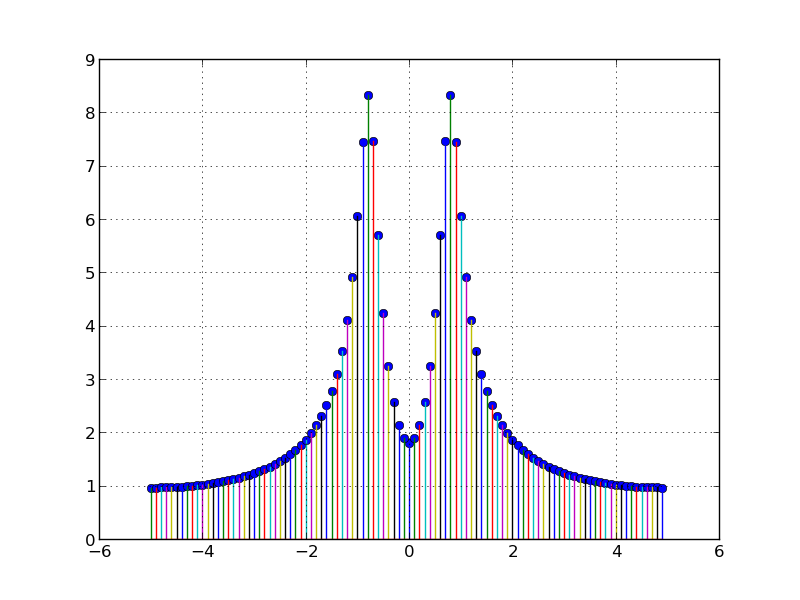
\includegraphics[width=0.48\textwidth]{./figures/DFT_mode_7.png}
  }
  \caption{DFT results of input $z'$.}
  \label{dft}
\end{figure*}

\end{document}
